\section{Perfekte Eliminations-Reihenfolgen}
Um einen Ansatz zur Prüfung der Chordalität eines Graphen zu finden, benötigt man eine äquivalente Aussage, die in diesem Abschnitt hergeleitet werden soll.

\begin{definition}[Vollständiger Graph]
	Ein Graph \( G = \left( V, E \right) \) ist vollständig, wenn jedes Paar \( v, w \in V \) von Knoten durch eine Kante \( \left\lbrace v, w \right\rbrace \in E \) verbunden ist.\footnote{siehe \cite[Kapitel 1.1]{golumbic}}
\end{definition}

Die \textit{Adjazenzmenge} eines Knoten \( x \in V \) bezüglich eines ungerichteten Graphen \( G = \left( V, E \right) \) sei die Menge der Knoten, zu denen \( x \) im Graphen \( G \) eine Verbindung besitzt: \( \textnormal{Adj} \left( x \right) = \left\lbrace y \in V \mid \left\lbrace x, y \right\rbrace \in E \right\rbrace \). Für eine Menge von Knoten \( X \subseteq V \) ist diese \( \textnormal{Adj} \left( X \right) = \bigcup_{x \in X} \textnormal{Adj} \left( x \right) \). Der durch die Teilmenge \( X \subseteq V \) induzierte \textit{Teilgraph} \( G \left[ X \right] \) sei definiert als \( G \left[ X \right] = \left( X, \left\lbrace \left\lbrace v, w \right\rbrace \in E \mid v, w \in X \right\rbrace \right) \).

\begin{definition}[Simplizialer Knoten]
	Ein simplizialer Knoten \( v \) in einem Graphen \( G \) ist ein Knoten, dessen Nachbarn einen vollständigen Teilgraphen \( G \left[\textnormal{Adj} \left( v \right) \right] \) induzieren.\footnote{siehe \cite[Kapitel 4.2]{golumbic}}
\end{definition}

Für den Beweis der nächsten Lemmata benötigen wir folgendes Hilfskonstrukt:

\begin{definition}[Minimaler Knotentrenner]
	Ein Knotentrenner \( S \) der Knoten \( a, b \in V \) ist eine Teilmenge \( S \subseteq V \) mit \( a, b \not\in S \), bei dem sich \( a \) und \( b \) in verschiedenen Zusammenhangskomponenten von \( G \left[ V \setminus S \right] \) befinden.

	\( S \) ist ein minimaler Knotentrenner, falls diese Aussage für kein \( T \subsetneq S \) gilt.\footnote{siehe \cite[Kapitel 4.2]{golumbic}}
\end{definition}

Das folgende Lemma stellt eine bestimmte Eigenschaft von chordalen Graphen dar, die wir in den darauf folgenden Beweisen benötigen:

\begin{lemma}
	Sei \( G = \left( V, E \right) \) ein chordaler Graph. Dann ist der induzierte Teilgraph \( G \left[ S \right] \) zu jedem minimalen Knotentrenner \( S \subseteq V \) vollständig.\footnote{siehe \cite[Satz 4.1 (i) \( \Rightarrow \) (iii)]{golumbic}}
	\label{theorem:seperator}
\end{lemma}

\begin{proof}
	Sei \( S \) ein minimaler Knotentrenner für die Knoten \( a \) und \( b \). \( G \left[ A \right] = \left( A, E_A \right)\) und \( G \left[ B \right] = \left( B, E_B \right)\) seien die Zusammenhangskomponenten von \( G_{V \setminus S} \), die jeweils \( a \) und \( b \) enthalten.

	Da \( S \) minimal ist, hat jeder Knoten \( v \in S \) jeweils einen Nachbarn in \( A \) und \( B \).
	Deshalb existiert zu jedem Knotenpaar \( x, y \in S \) ein minimaler Weg (bezüglich Kantenanzahl) \( \left( x, a_1, a_2, \ldots a_r, y \right) \) mit \( a_i \in A \) und \( \left( y, b_1, b_2, \ldots b_t, x \right) \) mit \( b_i \in B \).

	Der Kreis \( \left( x, a_1, a_2, \ldots, a_r, y, b_1, b_2, \ldots, b_t, x \right) \) besitzt mindestens die Länge \( 4 \) und hat somit, da \( G \) chordal ist, eine Sehne.
	Da die Wege minimal gewählt sind, kann diese jedoch nicht zwei Knoten aus demselben Weg verbinden, womit \( \left\lbrace a_i, a_j \right\rbrace \not\in E\) für \( i, j \in \left\lbrace 1, \ldots r \right\rbrace, \left| i - j \right| > 1 \) und \( \left\lbrace b_i, b_j \right\rbrace \not\in E \) für \( i, j \in \left\lbrace 1, \ldots, t \right\rbrace, \left| i - j \right| > 1 \) gilt. Da alle \( a_i \) und \( b_i \) durch \( S \) getrennt sind, ist außerdem \(\left\lbrace a_i, b_j \right\rbrace \not\in E \) für \( i \in \left\lbrace 1, \ldots, r \right\rbrace \) und \( j \in \left\lbrace 1, \ldots, t \right\rbrace \). Damit müssen die beiden Knoten \( x \) und \( y \) aus dem Knotentrenner verbunden sein.
\end{proof}

Mithilfe von Lemma \ref{theorem:seperator} können wir nun auch folgende Aussage treffen:

\begin{lemma}
	Jeder chordale Graph \( G = \left( V, E \right) \) besitzt einen simplizialen Knoten. Falls \( G \) nicht vollständig ist, dann besitzt dieser zwei nicht-benachbarte simpliziale Knoten.\footnote{siehe \cite[Lemma 4.2]{golumbic}}
	\label{theorem:simplicial}
\end{lemma}

\begin{proof}
	%TODO: Begründen, warum dieser Teilgraph wieder chordal ist

	\begin{itemize}
		\item[Induktionsvoraussetzung:] Für jeden Graphen \( G = \left( V, E \right) \) mit \( \left| V \right| \leq t \) gelte, dass \( G \) entweder vollständig ist oder zwei nicht-benachbarte simpliziale Knoten besitzt.
		\item[\( t = 1 \)] Da ein Graph bestehend aus nur einem Knoten vollständig ist, gilt der Induktionsanfang.
		\item[\( t \Rightarrow t + 1 \)]
		      Sei \( G = \left( V, E \right) \) ein Graph mit \( \left|
		      V \right| = t \) Kanten. Falls \( G \) vollständig ist, ist die Aussage trivial.

		      Habe \( G \) also nun zwei nicht-benachbarte Knoten \( a \) und \( b \) und die Aussage sei für alle Graphen mit weniger Knoten als \( G \) gültig. Wähle als \( S \) einen minimalen Knotentrenner von \( a \) und \( b \); \( G \left[ A \right] \) und \( G \left[ B \right] \) seien wie in Lemma \ref{theorem:seperator} definiert.

		      Wegen der Induktionsvoraussetzung gilt, dass entweder der Teilgraph \( G \left[ A \cup S \right] \) zwei nicht-benachbarte simpliziale Knoten besitzt, von dem einer in \( G \left[ A \right] \) liegen muss (da \( S \) nach Satz \ref{theorem:seperator} vollständig ist) oder \( G \left[A \cup S \right] \) vollständig ist.

		      Da \( \textnormal{Adj} \left( A \right) \subseteq A \cup S \), ist jeder simpliziale Knoten in \( G \left[ A \right] \) ebenfalls simplizial in gesamt \( G \). Mit einer ähnlichen Argumentation lässt sich zeigen, dass auch \( G \left[ B \right] \) einen simplizialen Knoten besitzt.
	\end{itemize}
\end{proof}

Um den Graphen auf Chordalität zu überprüfen, werden wir eine sogenannte perfekte Eliminations-Reihenfolge verwenden, die genau dann existiert, wenn \( G \) chordal ist. Eine \textit{Reihenfolge} ist dabei eine Bijektion \( \sigma: \left\lbrace 1, \ldots, \left| V \right| \right\rbrace \mapsto V \).

\begin{definition}[Perfekte Eliminations Reihenfolge]
	Eine Reihenfolge \( \sigma \) auf \( G = \left( V, E \right) \) ist eine perfekte Eliminations-Reihenfolge, wenn für jedes \( i \in \left\lbrace 1, \ldots, \left| V \right| \right\rbrace \) der Knoten \( \sigma \left( i \right) \) simplizial im Teilgraph \( G \left[ \left\lbrace \sigma \left( i \right), \ldots, \sigma \left( \left| V \right| \right) \right\rbrace \right] \) ist.\footnote{siehe \cite[Kapitel 4.2]{golumbic}}
\end{definition}

\vspace{1em}
\begin{minipage}{\linewidth}
	\centering
	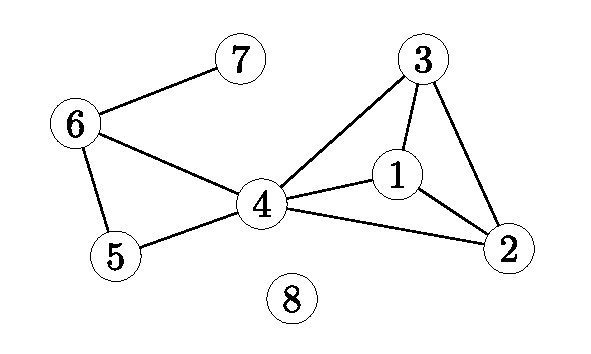
\includegraphics[scale=0.9]{img/graph/peo.pdf}
	\captionof{figure}[Perfekte Eliminations-Reihenfolge]{Die durch die Beschriftung der Knoten dargestellte Reihenfolge \( \sigma \) ist eine perfekte Eliminations-Reihenfolge.}
	\label{fig:peo}
\end{minipage}

Nun ist es uns möglich, die gesuchte Äquivalenz zu beweisen und damit die Hauptaussage des Abschnitts zu zeigen:

\begin{theorem}
	Sei \( G \) ein ungerichteter Graph. \( G \) ist chordal genau dann, wenn für \( G \) eine perfekte Eliminations-Reihenfolge \( \sigma \) existiert.\footnote{siehe \cite[Satz 4.1 (i) \( \Leftrightarrow \) (ii)]{golumbic}}
	\label{theorem:chordalpeo}
\end{theorem}

\begin{proof}
	\begin{itemize}
		\item[\(\Rightarrow\)]
		      Nach Satz \ref{theorem:simplicial} besitzt ein chordaler Graph \( G \) einen simplizialen Knoten \( x \). Da auch \( G \left[ V \setminus \left\lbrace x \right\rbrace \right] \) chordal ist und weniger Knoten als \( G \) besitzt, lässt sich induktiv eine perfekte Eliminations-Reihenfolge erstellen, wenn \( \sigma \) als Reihenfolge der in jedem Schritt entfernten \( x \) gebildet wird.

		\item[\(\Leftarrow\)]
		      Sei \( C \) ein Kreis in \( G \) mit mindestens vier Knoten und \( x \) der kleinste Knoten darin bezüglich \( \sigma^{-1} \left( x \right) \).

		      Durch die Wahl von \( x \) liegt \( C \) vollständig in \( G \left[ \left\lbrace \sigma \left( i \right) \mid i \geq \sigma^{-1} \left( x \right) \right\rbrace \right] \). Da der Knoten \( x \) in diesem Teilgraphen simplizial ist muss zwischen den beiden Nachbarknoten \( v, w \) von \( x \) im Kreis \( C \) eine Sehne existieren.
	\end{itemize}
\end{proof}
